\chapter[Introdução]{Introdução}
A prova de conceito da aplicação será composta pelo cadastro e acesso da aplicação por um Administrador. Este processo, conforme demonstra a Figura 1, consiste em: criar o usuário administrador, fornecendo e-mail e nome, utilizando um usuário administrador previamente criado, acessar o link que foi enviado para o e-mail, fornecer senha e confirmação de senha. E assim que clicar no botão, além de criar o acesso, estará dentro da plataforma.

\begin{figure}[htb]
    \centering
	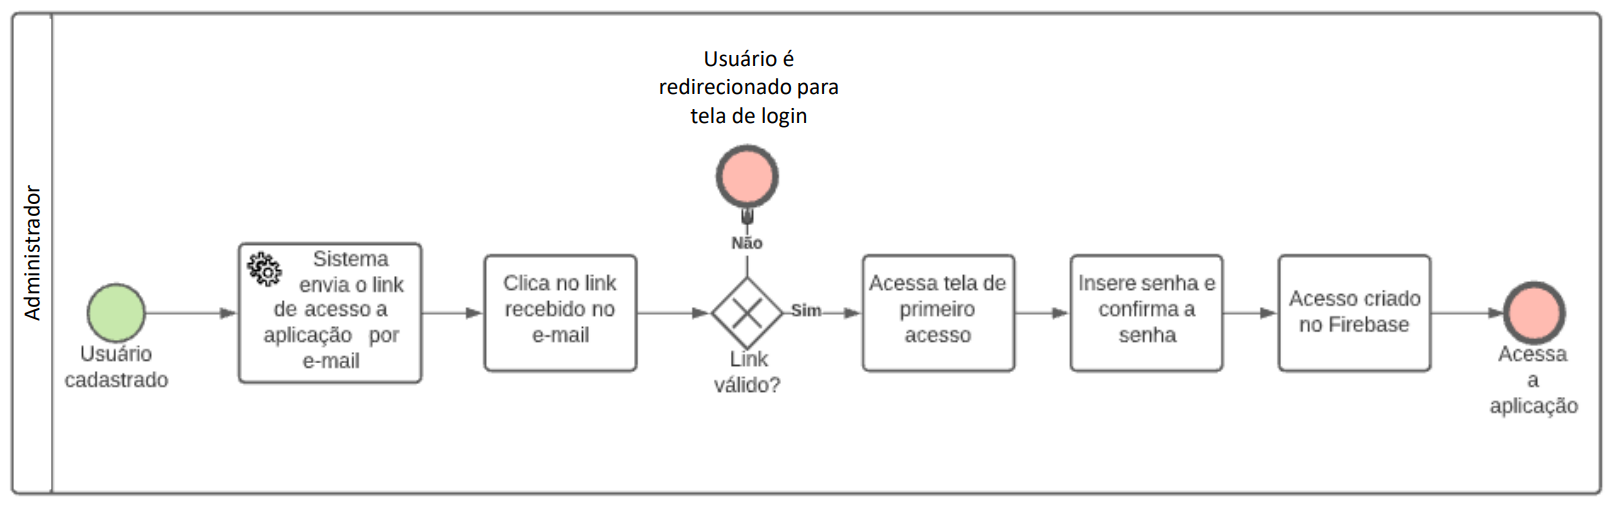
\includegraphics[width=16cm]{imagens/PrimeiroAcesso.png}
	\caption{Processo de Primeiro Acesso}
	\fonte{Os autores}
\end{figure}
\FloatBarrier

Caso o administrador já tenha sido cadastrado no sistema, basta realizar o processo de login na aplicação, conforme demonstrado na Figura 2.

\begin{figure}[htb]
    \centering
	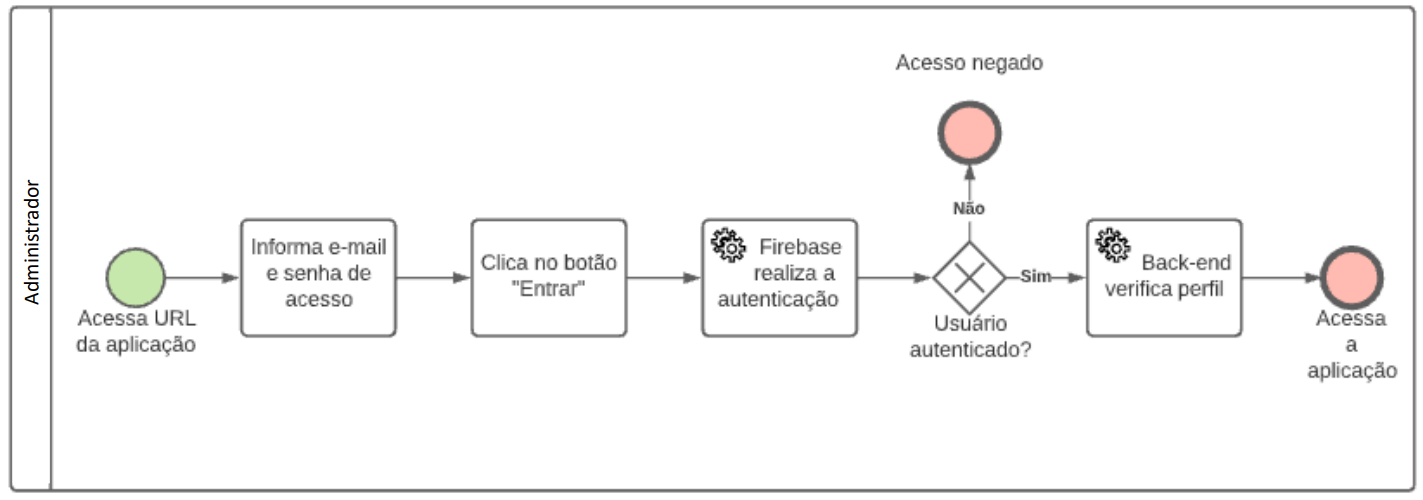
\includegraphics[width=16cm]{imagens/Login.png}
	\caption{Processo de Login}
	\fonte{Os autores}
\end{figure}
\FloatBarrier


Para que este processo possa ser concluído, todas as peças da arquitetura, conforme mostra a Figura 3, devem estar operando corretamente. A fim de simplificação, será considerado que pelo menos um usuário já foi cadastrado (o processo de cadastro do primeiro usuário é manual, realizando de forma direta a gravação da tupla no banco de dados e criação da URL de primeiro acesso). O início deste processo é através da interface web do projeto, escrita utilizando Angular 12 e servida através do Firebase Hosting.

\begin{figure}[htb]
    \centering
	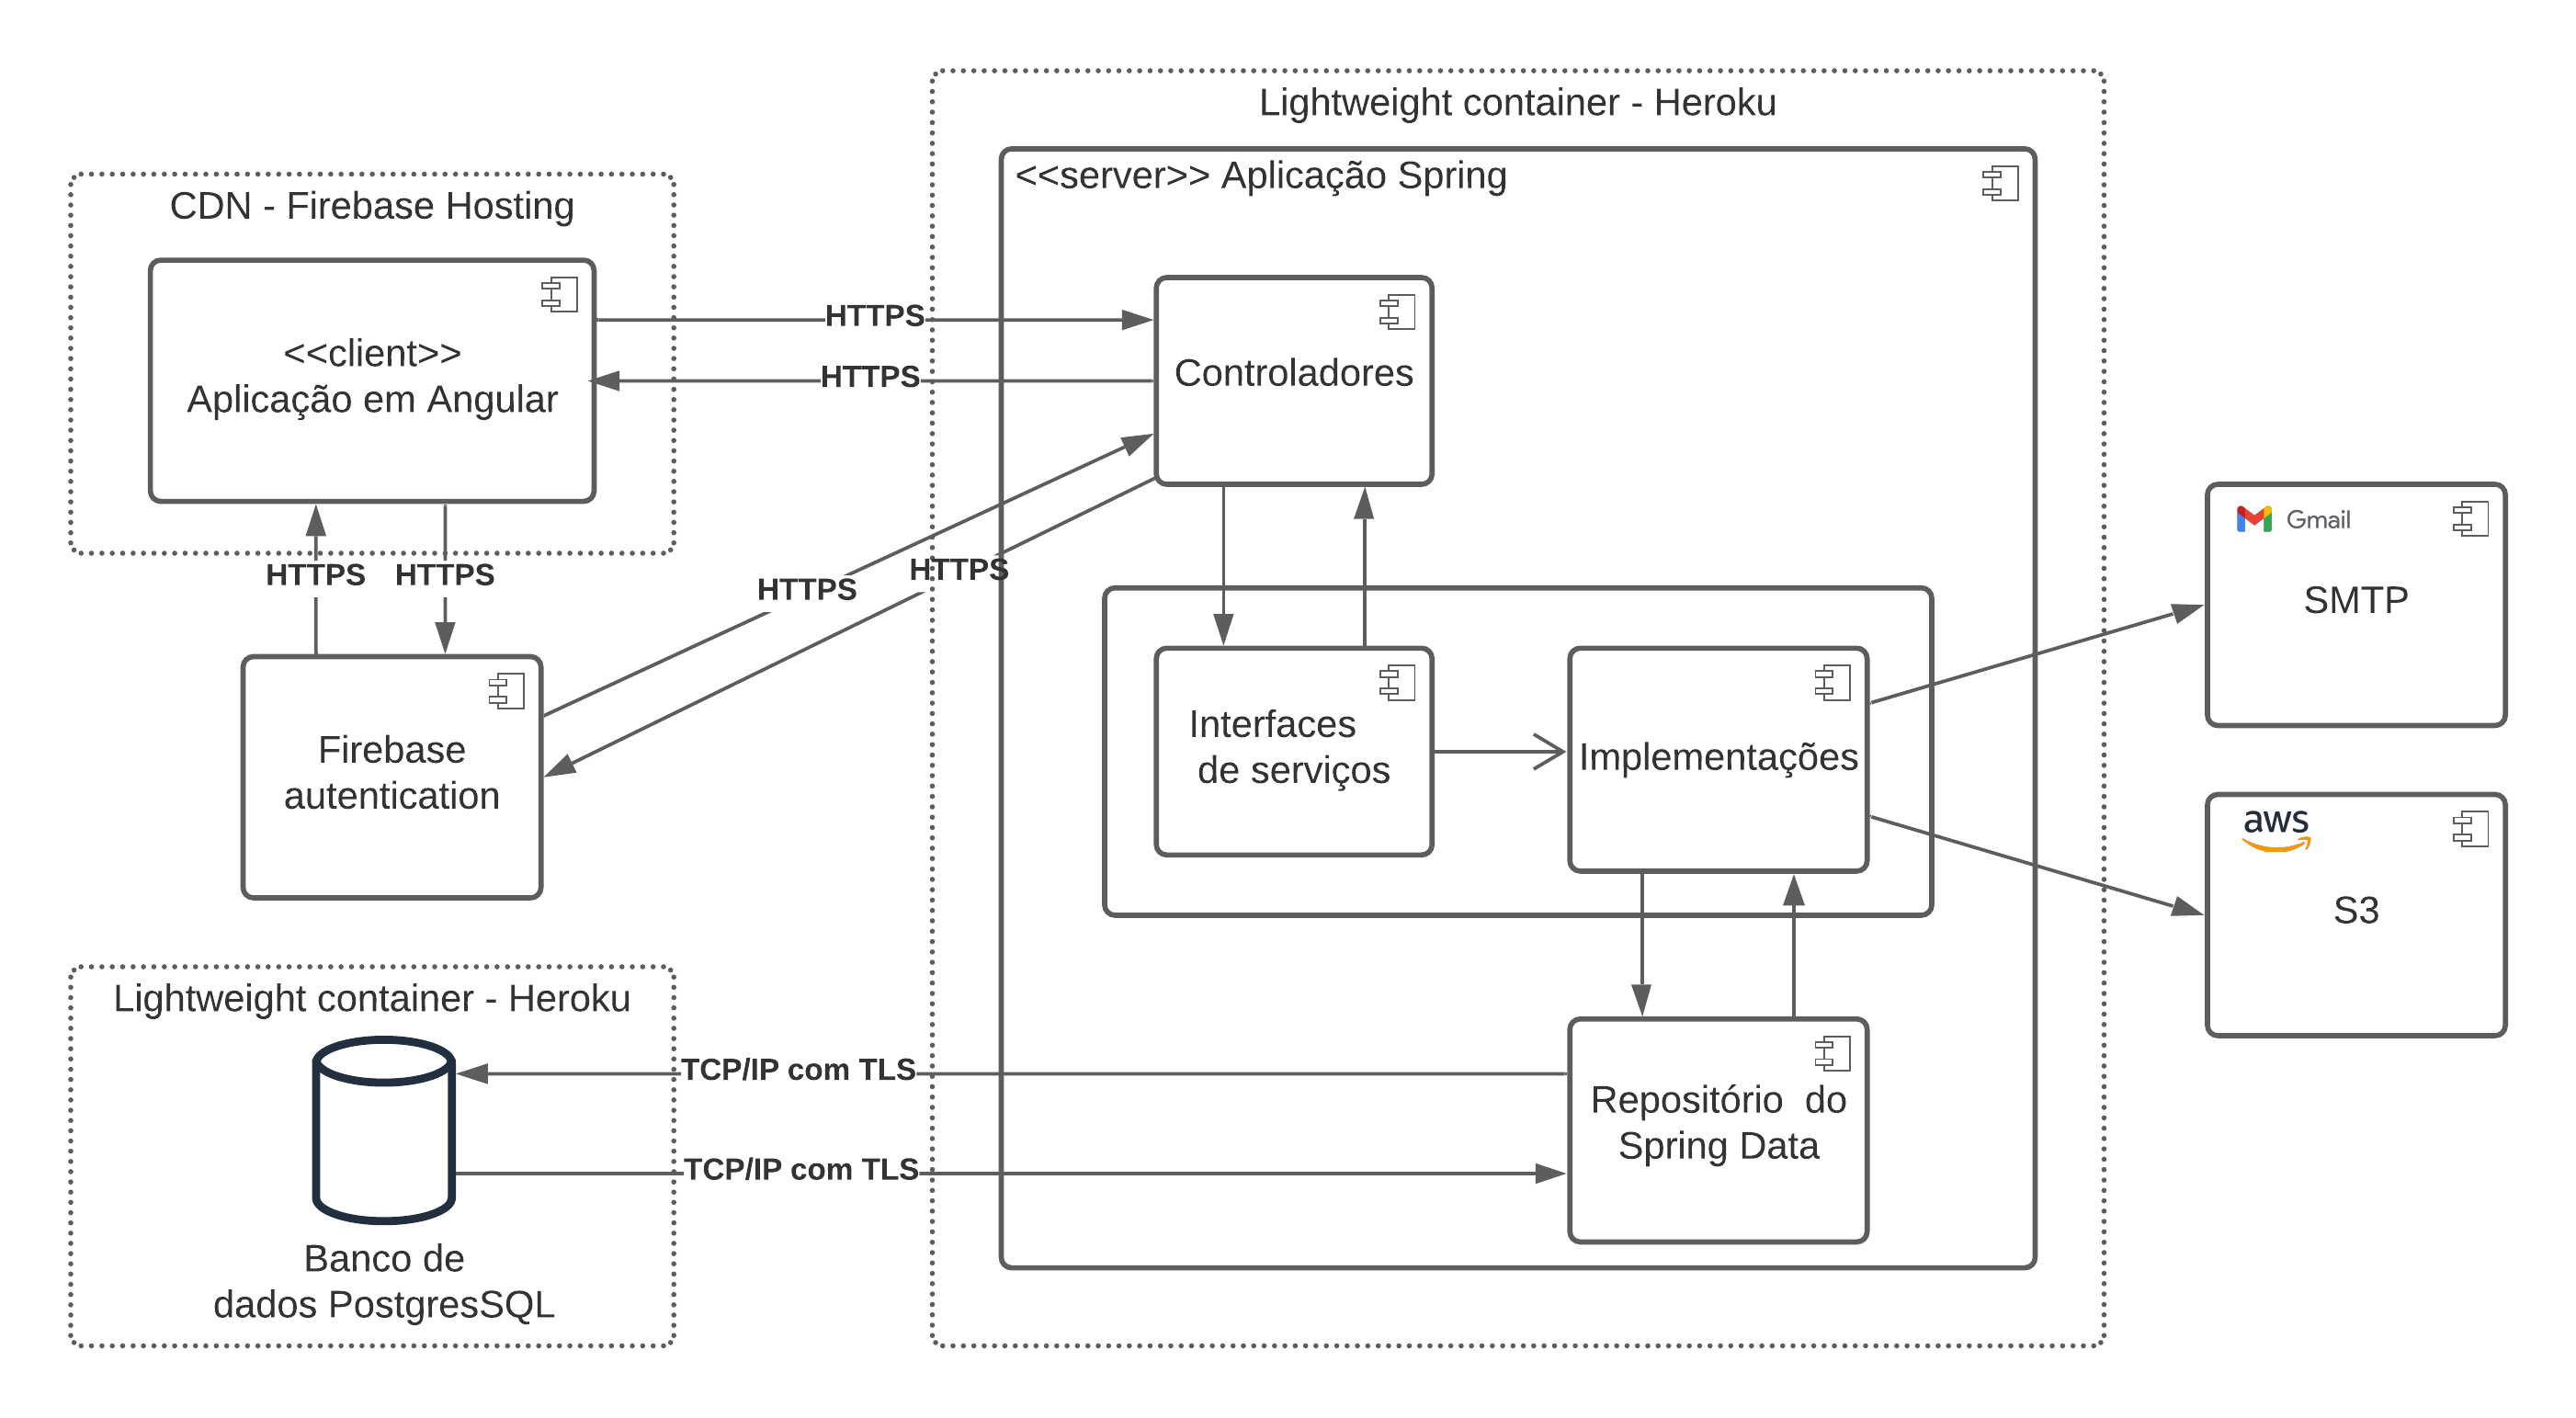
\includegraphics[width=16cm]{imagens/Arquitetura.png}
	\caption{Arquitetura da solução}
	\fonte{Os autores}
\end{figure}
\FloatBarrier

O projeto Angular foi criado utilizando a sua CLI (Command Line Interface) e o deploy no Firebase Hosting configurado utilizando a CLI do Firebase e realizada pelo Travis CI. Além disso, toda a interface foi construída utilizando o Angular Material Components, uma biblioteca de componentes que implementa o Design System Material Design, promovendo uma consistência de interface.

No momento que o usuário acessar a URL de login da aplicação, ele vai inserir o seu usuário e senha e realizar o login. O login da aplicação consiste em uma autenticação no lado cliente utilizando o @angular/fire, no qual a senha e e-mail são enviados para os servidores do Firebase. O cliente recebe de volta tokens que o identificam, e um destes tokens são utilizados para acessar endpoints protegidos do back-end.

O back-end é uma aplicação Java, escrita utilizando o framework Spring com as bibliotecas do ecossistema, hospedado em um dyno do Heroku. Este back-end também utiliza o MySQL para armazenar os dados pertinentes a aplicação, que está hospedado em um VPS da Oracle Cloud. Ele também utiliza a biblioteca de API de administração do Firebase (SDK Admin), que é utilizada tanto para autenticar usuários (verificando os tokens gerados para o cliente) quanto para criar os usuários (para que eles possam recuperar estes tokens no cliente).

Assim que o cliente concluir a autenticação do seu lado, ele realiza uma chamada ao back-end para verificar o papel do usuário e encaminhar para a interface adequada ao seu papel. Ao acessar a funcionalidade de criação do Administrador e criar o administrador, a requisição é enviada ao back-end, que realiza a requisição do envio de um e-mail com as informações de primeiro acesso. O envio de e-mail é realizado utilizando o servidor SMTP do Google, que é acessado utilizando as credenciais de um Gmail e Spring Email.

Quando o e-mail é recebido, o usuário que foi cadastrado, pode acessar o link, informar uma senha e então, um usuário será criado no Firebase Authentication, permitindo que este usuário possa acessar a plataforma
